\documentclass[10pt]{article}
\usepackage[margin=0.8in,top=0.7in,bottom=0.7in]{geometry}
\usepackage{amsmath}
\usepackage{booktabs}
\usepackage{graphicx}
\usepackage[hidelinks]{hyperref}
\usepackage{xcolor}
\usepackage{parskip}

\graphicspath{{../results/stack/}}
\makeatletter
\renewcommand\section{\@startsection{section}{1}{\z@}{8pt}{3pt}{\normalfont\large\bfseries}}
\makeatother
\setcounter{secnumdepth}{0}
\setlength{\leftmargini}{1.2em}
\pagestyle{empty}

\begin{document}

{\LARGE\bfseries Can we pick training data so that a circuit forms early?}\\[2pt]
{\large A research project on how circuits form in small transformers and how to select data for them}\\[2pt]
{\small Research summary, Luca Columbu, 2026. Full draft and code: \textcolor{red}{[link]}.}

\section{What we wanted to know}
A language model learns its abilities as small internal \emph{circuits}:
groups of attention heads and neurons that together perform one
computation. We wanted to understand how one such circuit forms during
training, which properties of the training data make it form sooner or
later, and whether we could then \emph{choose} training data so that the
circuit forms earlier, or with less data, than it would on a random
sample of the same corpus.

Today's data-selection methods (filtering by loss, matching a target
distribution, removing duplicates) score each document with one number
that mixes every ability together. They cannot say which ability a
decision helps or hurts, because they never look at what the model builds
inside. We wanted a score aimed at one specific circuit.

\section{The circuit we chose, and the trick}
We chose the \emph{induction head}, the best-understood circuit in
transformers and the one behind in-context learning. Its job is simple:
when the model sees a token it has seen before in the current context,
it looks back to that earlier occurrence and predicts whatever followed
it last time. If the context contains ``Mr Dursley \ldots\ Mr'', it
predicts ``Dursley''.

The trick is that this is also exactly what the \texttt{gzip} compressor
does. Its LZ77 algorithm finds the earlier occurrence of the current
string and replaces the repeat with a pointer to it. So we can use
\texttt{gzip} as a stand-in for the circuit: a document that compresses
well because of repeated passages is a document that would exercise an
induction head. Our score for each document is its \emph{compression
gain}: how much shorter it compresses than a shuffled copy of itself
(the shuffle keeps the word counts, so only genuine repeated structure
counts). The score is free to compute and needs no model.

\section{How we tested it}
\begin{enumerate}
\item \textbf{Built synthetic tasks with adjustable knobs.} Random token
  sequences with an embedded repeat, where we control how much is
  repeated, how long the copies are, how noisy the data is, and how big
  the vocabulary is. Each setting is a different training set with a
  different compression gain.
\item \textbf{Trained small transformers (2 to 4 layers) and recorded
  when the circuit forms.} We saved checkpoints every 100 steps and, at
  each one, measured whether the induction head exists (does a head
  attend to the right earlier token, and does patching its output into
  a corrupted run restore the answer) and whether the model copies
  correctly. The ``formation step'' is where these cross a threshold.
  Three seeds per setting; about 200 runs in total.
\item \textbf{Checked the prediction.} Does a dataset's compression gain
  tell us, before training, when the circuit will form?
\item \textbf{Used it to select data.} Took a mixed pool of documents,
  kept a fixed-size subset by gain, trained on it, and compared with a
  random subset of the same size and with an oracle that sees the hidden
  generating parameters.
\item \textbf{Repeated the selection on real data.} 2.5 billion tokens
  of Python code from The Stack, on a rented GPU.
\end{enumerate}

\section{What we found}
\begin{itemize}
\item \textbf{The score predicts when the circuit forms.} Across the
  synthetic settings, higher compression gain means earlier formation,
  almost perfectly in rank (Spearman $-0.98$ for attention-only models,
  $-0.92$ with MLPs, $-1.0$ on condition averages). The circuit arrives
  as a sudden jump, and the jump's timing follows the score, not the
  nominal amount of repetition we had dialled in.
\item \textbf{Selecting by the score forms the circuit much earlier with
  a third of the data.} From a pool of 60,000 documents, the 20,000 with
  the highest gain form the circuit at step 700 in every seed. A random
  20,000 forms it at step 5,200 or not at all. The score beat even the
  oracle (800--1,000): the oracle knows how much repetition was
  \emph{requested} for each document, the compressor measures how much
  was actually \emph{produced}.
\item \textbf{The data decides which version of the circuit forms.} We
  expected one circuit; we found a family. Depending on how long the
  copies in the data are, the model builds an induction head that looks
  $k$ tokens behind the ideal position, and that choice caps its
  accuracy. Training curves that looked like partial learning were
  finished circuits of the ``wrong'' variant. We traced this to a simpler
  positional circuit the model builds first and then grows the induction
  head on top of.
\item \textbf{Where the score fails, a small model can take over.} With a
  tiny vocabulary, accidental repeats fool the compressor. Replacing
  \texttt{gzip} with a small model that already has an induction head
  restores the prediction. The compressor is a hand-written version of
  the circuit; a trained model is a learned one.
\item \textbf{Repetition within a document and variety across documents
  are different things.} A second score, the compression
  \emph{distance} between documents, measures variety. It does not
  predict formation, but it relates to how well a second task's circuit
  generalises to unseen combinations. The two scores pull in opposite
  directions when selecting, which matters below.
\end{itemize}

\section{On real code}
From 2.5B tokens of Python (9.77M windows of 256 tokens) we selected a
fifth by gain, with a variety constraint so that near-duplicate
boilerplate is skipped, and compared it with a random fifth. Same
4-layer model, same 491M training tokens, three seeds each; one seed per
arm continued to 983M.

\begin{center}\small
\begin{tabular}{lcccc}\toprule
Training data & Head forms (step) & Model copies correctly (step) & Final copy accuracy & Validation loss \\\midrule
Selected by score & 1,000 in every seed & 2,000 in every seed & 0.84--0.86 & 1.78--1.80 \\
Random & 1,500--2,000 & 4,000--6,000 & 0.70--0.78 & 1.59--1.61 \\\bottomrule
\end{tabular}
\end{center}

\begin{center}
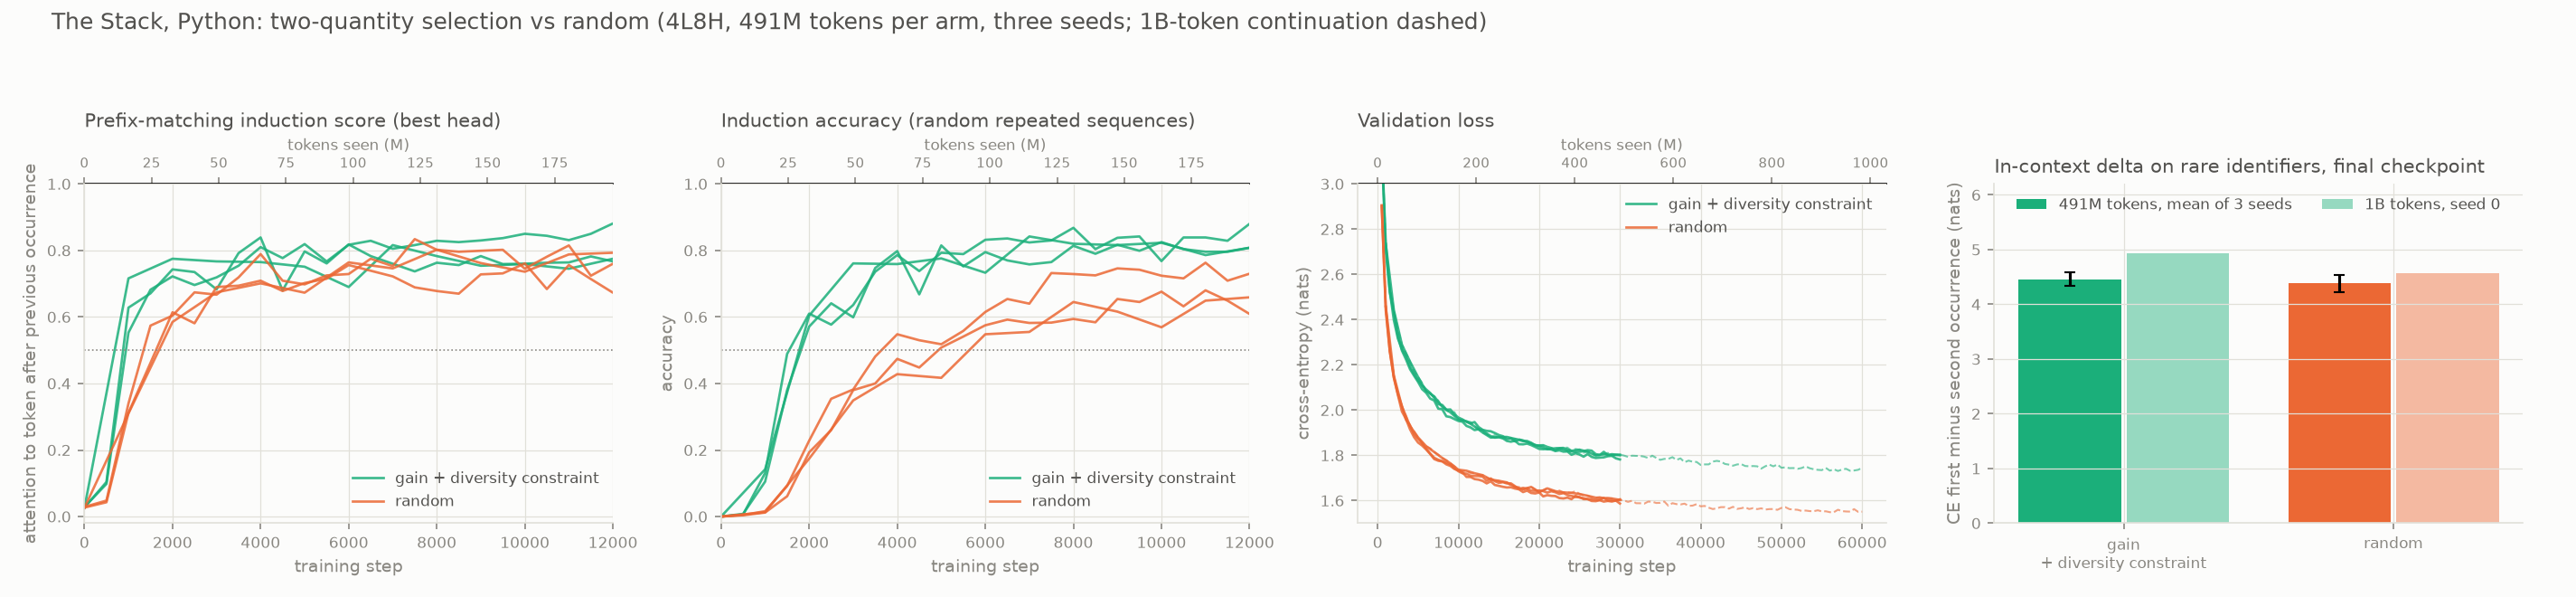
\includegraphics[width=\textwidth]{stack_trajectories.png}
\end{center}

The selected data forms the induction head 1.5 to 2 times sooner and
the copying behaviour 2 to 3 times sooner, in every seed, and the
model keeps copying more accurately to the end. The cost is visible in
the last column: the model trained on selected data is a worse general
language model by 0.2 nats, because the most repetitive fifth of a corpus
is a narrower slice of it, and doubling the training budget does not
close that gap. Once both models have the circuit, a test on rare
variable names (how much cheaper the second occurrence is than the
first) shows they use it equally well. So selection by this score buys
\emph{when} the circuit forms, and the second score, variety, is what
limits the price. A smaller study with four selection strategies showed
the trade-off can be tuned: gain buys the circuit, variety buys the
distribution.

We also learned to tell in advance where the method cannot work. On
children's stories, long repeated passages cover under 0.4\% of tokens,
the score has nothing to grip, and no induction head formed in any run.
The compressor's own match-length statistics predicted that before we
trained anything.

\section{What this involved}
Everything was built from scratch in Python with PyTorch and
TransformerLens: the task generators, the training and checkpointing
code, the circuit measurements (attention patterns, exact logit
attribution, activation patching, minimal sufficient head sets), the
scores, the selector, and a streaming pipeline for The Stack. A habit
that paid off: trace what one trained model actually does before running
a sweep. Three times this caught a model solving the task by a shortcut
that would have given clean-looking results about the wrong circuit, and
the task was redesigned each time. Almost all runs fit on a laptop; the
real-data study cost about \$7 of rented GPU time.

\section{What is still open}
Models are small (2 to 4 layers), one circuit family is covered, and the
formation steps are early compared with production training budgets. We
have not shown selection working on prose, and the natural next step is
a circuit where the compressor should fail and a learned score should
take over: facts stated in several paraphrases.

\end{document}
